\section{Uživatelská aplikace}\label{sec:tvorba-gui-rozhrani}
Na začátku této práce jsem si v kapitole(~\ref{ch:tvorba-zadani}) identifikoval požadavky, které by měl systém Coopmaster plnit.
V této části se podíváme na funkctionalitu z pohledu uživatelského rozhraní.

Pro implementaci jsem, po prvních pokusech s vlastní aplikací, zvolil open source systém pro chytré domácnosti Home Assistant~(\ref{sec:home-assistant}).
Mezi jeho hlavní výhody patří robustnost, konfigurace, integrovatelnost a široká možnost vizualizace dat.
Vytvořit takto robustní a kvalitní uživatelské rozhraní by za mě trvalo velmi dlouho a to nepočítám čas na jeho odladění a připadné opravy.

\subsection{Požadavky na systém}

\subsubsection*{Vzdálený přístup}
Má Home Asistant podporu pro vzdálený přístup? Odpoved je ano.
Home Assistant umožňuje vzdálený přístup, což uživatelům dovoluje řídit a konfigurovat jejich chytrou domácnost odkudkoli.
Pokud se provozuje system v cloudu, je to výrazně jednodušší.
V mém případě Home Assistant běží lokálně na stroji a je přístupný pouze z lokální sítě.
Tuto drobnost jsem vyřešíl konfigurací využijeme privátního tunelu, který poskytuje například společnost Cloudflare~\cite{cloudflare}.

Podrobně je výběr technologie pro vzdálený přístup popsán v sekci~\ref{sec:zpristupneni-aplikace-z-internetu}.

Při své práci jsem systém Home Assistant využival již od začátku skrze webové rozhraní a mohu tedy potvdit, že práce s ním je příjemná a vyhovující.
Vzdáleným přístupem tedy systém disponuje a nemusíme ho tedy nijak složitě implementovat.

%todo ozdrojovat cloudflare
%todo zdroj pro mqtt image https://www.home-assistant.io/integrations/image.mqtt/

\subsubsection*{Pohledy z bezpečnostních kamer}
Zobrazování obrázků z kamer je jednou ze základních komponent, kterou HomeAssistant nabizi.
Stací si vybrat komponentu, která bude schopna zpracovat data z MQTT serveru.
Ja jsem si vybral komponentu Picture.
Použil jsem pro ni defaultní konfiguraci, jen jsem ji nastavil attribute title, abych si na dashboardu odlišil přehledová data z výbehu a kurníku.
%todo odkaz na pouziti picture a mqtt entity pro obrázky

\subsubsection*{Dálkové ovládání a automatizaci světla a dvířek v kurníku}
Tímto bodem rozumíme v prvé řadě ovládací komponenty/tlačítka, která bude využívat chovatel, aby manuálně vyslal příkaz k provedení nějaké akce.
Za druhé se zde dostáváme k dalšímu skvělému využití systému Home Assistant a to je automatizace.
Využitím systému Home Assistant lze automatizovat právě reakce na hodnoty různých čidel a senzorů.
Může se jednat o automatizaci od úplných základů jako je zapnutí topení, když je v bytě zima, až po celé inteligentní domácnosti ovládané hlasem.
Takové domácnosti například na základě toho, kdo přišel domů, nastaví barvu světla, spustí jeho oblíbenou hudbu a uvaří kávu.
Já ve svém projektu využiji automatizaci k tomu, aby zavírala dvířka na základě času a počtu slepic, který poskytuje služba Chicken Watch Guard systému Coopmaster.
Dále pak automatizace na základě času zapíná a vypíná světlo.\newline
Pro splnění tohoto požadavku bude tedy třeba nakonfigurovat automatizaci a vytvořit ovládací tlačítka (obrázek~\ref{fig:homeassitant_lamp_button}).

\begin{figure}[H]
    \centering
    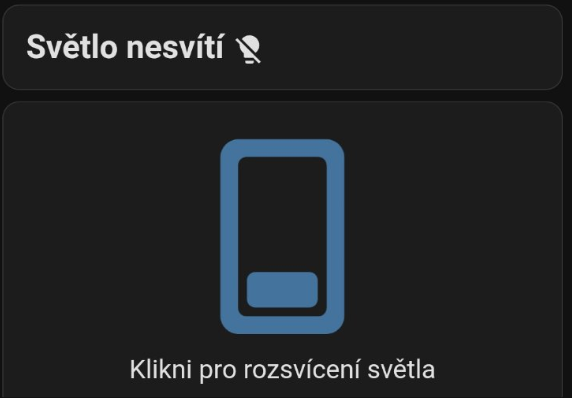
\includegraphics[width=0.8\textwidth]{img/homeasistant_lamp_button.png}
    \caption{Komponenta pro ovládání světel systému Home Assistant}
    \label{fig:homeassitant_lamp_button}
\end{figure}


%todo přidat odkaz na coopmaster a chicken guarda a na dokumentaci home assistant automatizace

\subsubsection*{Intuitivní vizualizace stavů jednotlivých hnízd(sedící slepice, v opačném případě počet vajec)}
Tento bod je ze všech nejnáročnější.
Home Assistant totiž nedisponuje žádnou pěknou komponentou přímo pro vizualizaci hnízd v kurníku a ani žádnou jinou, která by se dala po nějakých úpravách využít.\newline
Z tohoto důvodu bude tedy třeba vytvořit vlastní komponentu pro systém Home Assistant, která půjde snadno parametrizovat dle požadavků kurníku a bude umět zpracovat data, která přijdou ze služby Nest Watcher systému Coopmaster.

\subsubsection*{Upozornění na detekování vetřelce ve výběhu}
Zde se bude opět jednat o automatizace.
Požadavkem je, aby v případě poplachu systém poslal notifikaci chovateli a zobrazil na dashboardu aktuální fotografii, kde byl vetřelec detekován.\newline
Abychom splnili tento bod, budeme muset nastavit automatizaci, která zareaguje na určitý stav nějaké MQTT entity a následně vytvoří notifikaci.
Tato notifikace vyskočí i na chovatelově telefonu.
Dále bude použita komponenta s názvem Conditional, která umožnuje na základě hodnoty, měnit vizualizaci komponent na dashboardu.
Pri určitém stavu MQTT entity zobrazí v dashboardu upozornění na vetřelce ve výběhu a opačném případě nezobrazí nic.
Což je velmi šikovné právě pro různá upozornění.
%//todo odkaz na komponentu conditional

\subsubsection*{Data o teplotě a vlhkosti}
Tyto dva požadavky nebudou, co do implementace nic složitého.
Jedná se pouze o dvě hodnoty, které navíc ze služby Room Assistant chodí ve formátu JSON, takže není problém je zpracovat.\newline
Bude tedy třeba jen nakonfigurovat MQTT entitu, kterou následně bude načítat komponenta Entities.
Tato komponenta zobrazuje v seznamu pod sebou entity, jejichž seznam přebírá jako parametr.
Pro zobrazení každé entity je možno upravit ikonu a zobrazovaný název, což přesně odpovídá našim požadavkům.
%todo odkaz na kompoentu entities

\subsection{Postup konfigurace systému Home Assistant}
Po rozvržení řešení jsem se začal seznamovat se systémem Home Assistant s čímž mi hodně pomohla rozsáhlá a kvalitní dokumentace společně s diskusními fóry, která jsem hojně využíval.
\subsubsection*{MQTT entity}
Konfiguraci jsem započal definováním všech potřebných MQTT entit v souboru configuration.yaml, do kterých systém ukládá data přijatá z MQTT brokeru a následně je můžeme využít v našem dashboardu.
Používám tři typy MQTT entit.
\begin{itemize}
    \item sensor - přijímá běžné hodnoty senzoru jako čísla a texty (maximální velikost je 255 bytů)
    \item image - umožňuje přijmout obrázek z MQTT brokeru
    \item binary\_sensor - na základě nakonfigurovaných hodnot je jeho stav buď 0 nebo 1
\end{itemize}
Každá MQTT potřebuje nastavit jednotnačné jméno pro identifikaci v systému a topic, ze kterého bude odebírat zprávy.

%todo ukazka na konfiguraci entit a na dokumentaci

\subsubsection*{Základní dashboard}
Jakmile se nakonfigurují entity, následuje tvorba samotného dashboardu.
Za pomocí webového rozhraní jsem tedy přidal tlačítka, vizualizace obrázků a výpisy hodnot entit tak, jak bylo rozebráno dříve v návrhu.
Po přidání komponent bylo třeba přiřadit odpovídající entity ke komponentám opět s využitím webového rozhraní.

\subsubsection*{Automatizace}
Díky intuitivnímu webovému rozhraní systému není problém přidat jakoukoli automatizaci.
Automatizaci si lze představit stejně jako klasickou podmínku v programování.
Je zde sekce Spouštěč, která nastavuje hlavní důvod spuštění automatizace.
Následuje volitelná sekce A Pokud.
Tato sekce udává další omezení pro spuštění scriptu.
Na závěr je zde sekce Pak Provést, která právě specifikuje akci nebo akce, které se mají uskutečnit při splnění podmínek.
S těmito vědomostmi jsem opět nakonfiguroval dle návrhu potřebné automatizace pro světlo, dvířka a notifikace.

%todo najít návod na přidávání automatizace a dat ho taky jako zdroj

\subsubsection*{Tvorba vlastní Home Assistant komponenty}
Zde se již dostáváme k opravdovému programování. Inspirací jak komponentu vytvořit mi byla developerská dokumentace~(\cite{homeassistant-developers}).
Služba Nest Watcher poskytuje data o tom zda je hnízdo obsazené a kolik je v každém hnízdě vajec.
Tato data jsou ve formátu CSV, kdy každý prvek v poli znamená jedno hnízdo.
Data se do komponenty dostávají z entit.
Tyto entity se nastavují jako parametry během přidávání komponenty na dashboard.
Data, která dostaneme z entity, jsou v CSV formátu, takže se pomocí funkce split rozdělí podle separátoru, kterým je v tomto případě znak středníku.
%todo dodat ukázky kodu
Skript pokračuje do další části, kde dochází ke zpracování naparsovaných dat.
Jednoduchými dvěma for cykly se zajišťuje vykreslování nastaveného počtu řádků a sloupců v kurníku.
Jedno hnízdo se vykresluje obarvený DIV a jeho child komponenta je DIV, který slouží k vizualizaci stavů hnízda.
Graficky jsou DIVy nastylovány tak, aby uživateli připomínali hnízdo.
Do child divu se následně vykreslí vpravo dole počet vajec, pokud je větší než 0, a zároveň se ve středu vykresluje ikonka slepice, která značí, že slepice sedí v hnízdě. (obrázek~\ref{fig:homeassitant_custom_component})
Komponenta také při každém updatu dat loguje do konzole pro případ, kdy by se něco pokazilo.

\begin{figure}[H]
    \centering
    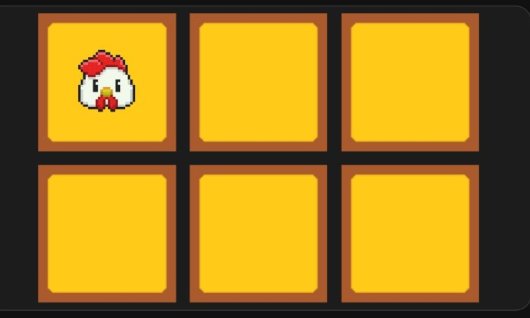
\includegraphics[width=0.8\textwidth]{img/homeassitant_custom_component}
    \caption{Vlastní komponenta pro systém Home Assistant}
    \label{fig:homeassitant_custom_component}
\end{figure}


%\subsection*{Problémy a poznatky během konfigurace}
%Během práce se systémem Home Assistant, jsem posbíral několik poznatků a narazil na několik problém.

\subsection*{Maximální velkost hodnoty senzoru}
Během tvorby komponenty pro hnízda, mě poněkud zaskočil fakt, že maximální velikost hodnoty state v entitě je 255 bytů.
Z počátku jsem chtěl posílat data o hnízdech ve formátu JSON.
Dlouho mi to procházelo, ale problém začal v situaci, kdy jsem serializoval celý seznam s objekty hnízd a chtěl ho poslat jako hodnotu senzoru.
Nebylo jednoduché na to přijít, protože v tomto případě Home Assistant data prostě nenačítal a já nevěděl proč.
Nakonec jsem se na diskusním fóru dočetl, že velikost hodnoty state je omezena.
Byl jsem tedy donucen začít používat formát CSV a posílaná data omezit pouze na nejnutnější informaci o stavu.
Pořád je zde problém s maximální velikostí v případě, že bych měl více než 128 hnízd, místo by mi i tak nevystačilo,
Na kontrolu tolika hnízd, bych ale potřeboval pravděpodobně o dost celkově robustnější infrastrukturu systému Coopmaster, takže to ponechávám ve formátu CSV.
%todo najít zdroj pro 255 bytů

%\subsubsection{Pozitivní zkušenost s tvorbou komponent}
%Práce na komponentě pro vizualizaci hnízd mi přinesla mnoho informací

\subsection*{Mobilní aplikace}
Mobilní aplikace Home Assistanta umožňuje uživatelům vzdáleně monitorovat a ovládat jejich inteligentní domácnost, poskytuje notifikace v reálném čase a nabízí přehledné uživatelské rozhraní pro snadnou správu zařízení a automatizací.

\begin{figure}[htbp]
    \centering
    \begin{minipage}[t]{0.5\textwidth}
        \centering
        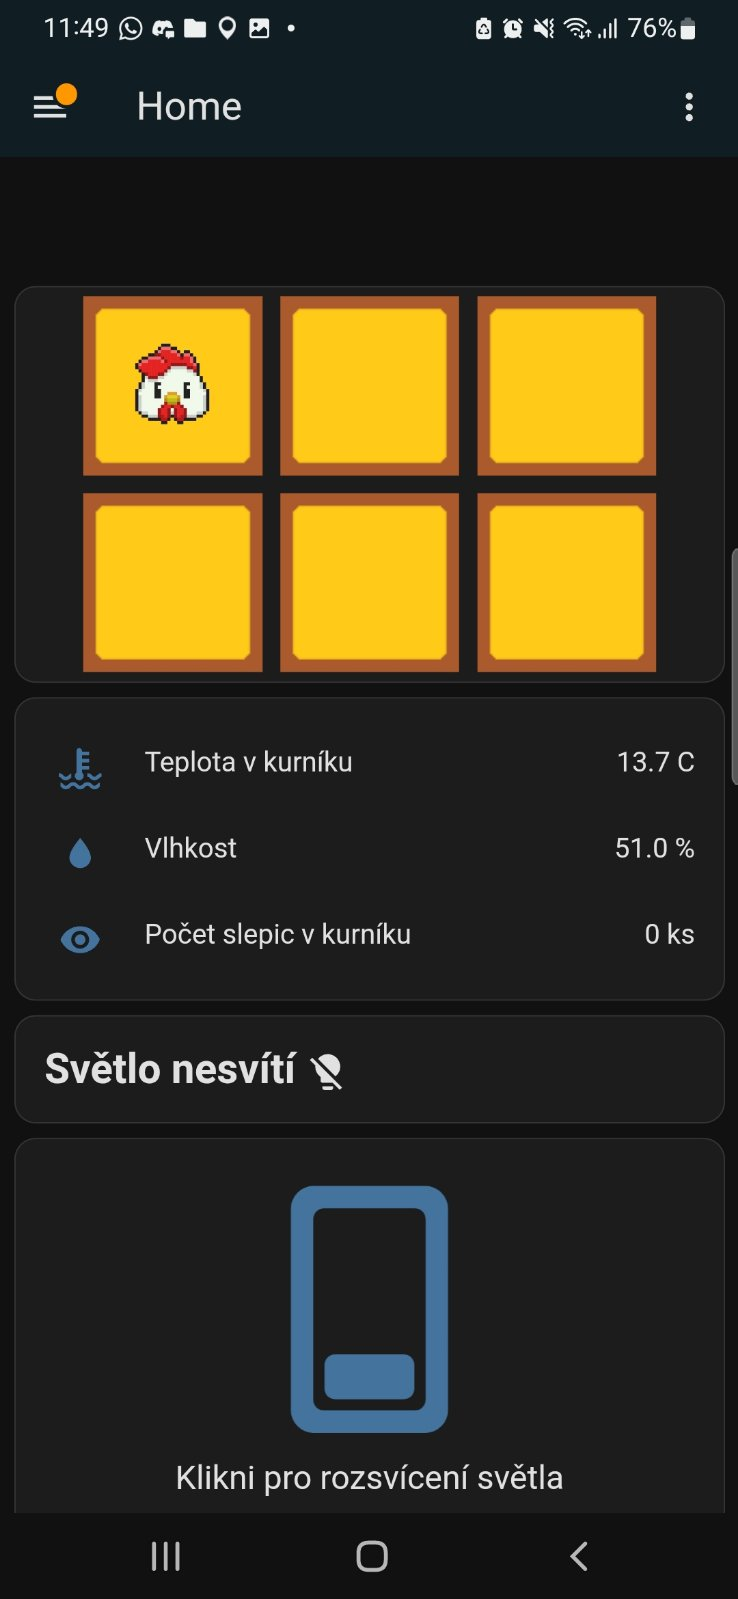
\includegraphics[width=0.9\textwidth]{img/mobilni_apka1}
        \label{fig:mobilni_apka1}
    \end{minipage}%
    \begin{minipage}[t]{0.5\textwidth}
        \centering
        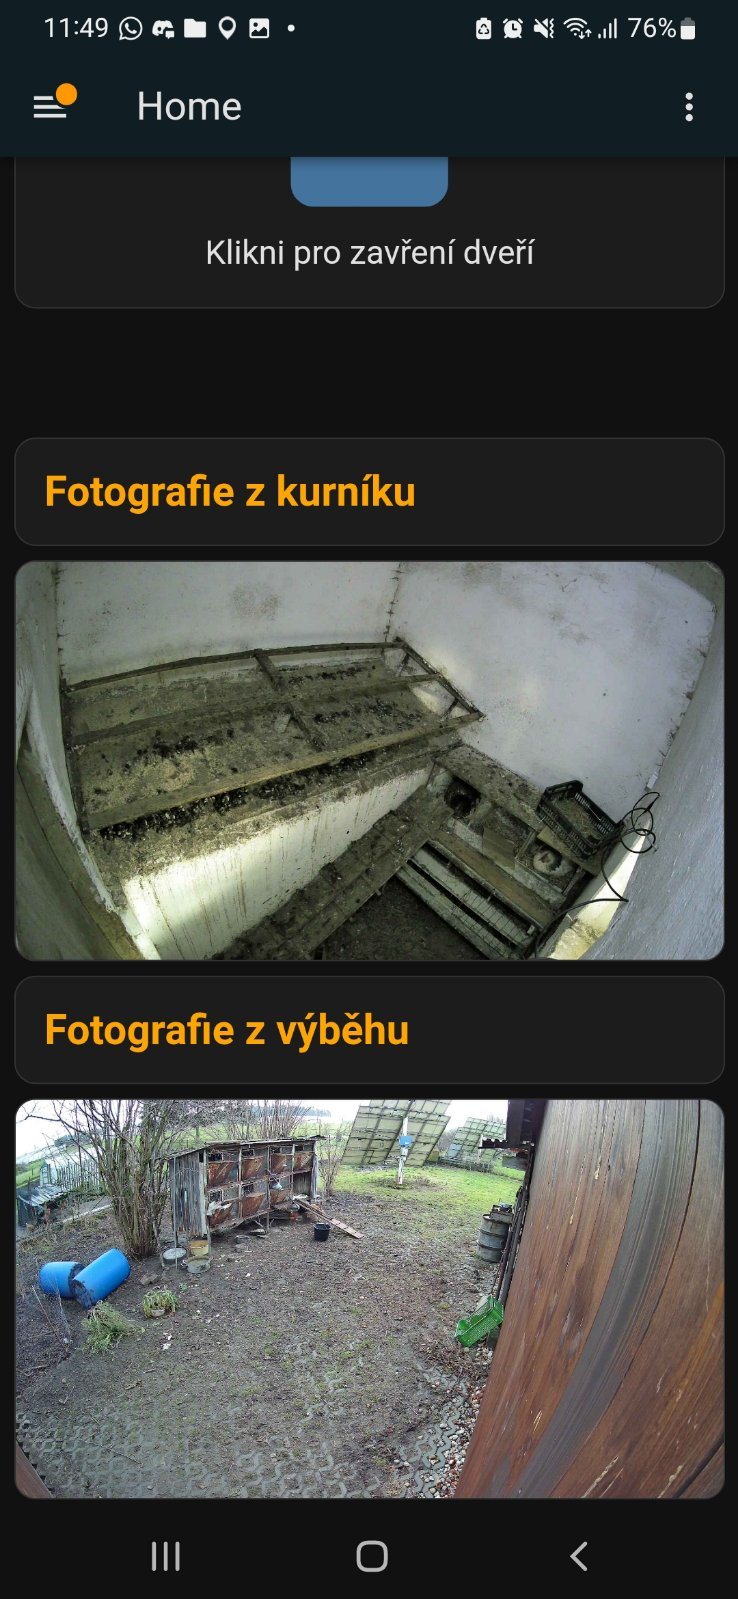
\includegraphics[width=0.9\textwidth]{img/mobilni_apka2}
        \label{fig:mobilni_apka2}
    \end{minipage}
    \caption{Mobilní aplikace Home Assistant}
\end{figure}

